%   ##
%
%   Band VIII, 3 N.~??A10.2
%   Signatur/Tex-Datei: LH_35_09_15_008-009
%   RK-Nr. 41152 [Teil 2]
%   Überschrift: Tentaminum de chordarum tensione scheda secunda
%   Datierung: 1680.12.10
%   WZ: 8-blättrige Rosette auf Zahl 80 (RK-WZ: 138)
%.  SZ: (keins)
%.  Bilddateien (PDF): LH_35_09_15_008-009_d1; LH_35_09_15_008-009_d2; LH_35_09_15_008-009_d3; LH_35_09_15_008-009_d4 (insgesamt vier)
%
%
\begin{ledgroupsized}[r]{120mm}
\footnotesize
\pstart
\noindent\textbf{Überlieferung:}
\pend
\end{ledgroupsized}
\begin{ledgroupsized}[r]{114mm}
\footnotesize
\pstart \parindent -6mm
\makebox[6mm][l]{\textit{L}}%
Aufzeichnung: LH~XXXV~9,~15 Bl.~8\textendash9.
Ein Bogen 4\textsuperscript{o};
ein Wasserzeichen im Falz.
Vier einspaltig beschriebene Seiten. 
\pend
\end{ledgroupsized}
%
%
\vspace{3.8mm}% !!!!! Vorläufig geändert !!!!!
%
%
\count\Bfootins=800
\count\Afootins=1000
\count\Cfootins=800
%
%
\pstart%
\normalsize%
\noindent%
%
\lbrack8~r\textsuperscript{o}\rbrack% Blatt 8r
%
\pend%
% Überschrift
\pstart%
\centering%
Tentaminum\protect\index{Sachverzeichnis}{tentamen} de chordarum tensione\protect\index{Sachverzeichnis}{tensio chordae}
\edtext{scheda\protect\index{Sachverzeichnis}{scheda} secunda 10 Xb.}{%
\lemma{scheda}\Bfootnote{%
\textit{(1)}~prim
\textit{(2)}~secunda
\textbar~10 \textit{erg.}~%
\textbar\ Xb.%
~\textit{L}}}
\edlabel{LH_35_09_15_008r_Anfg-1}%
1680
\edtext{}{{\xxref{LH_35_09_15_008r_Anfg-1}{LH_35_09_15_008r_Anfg-2}}{%
\lemma{1680}\Bfootnote{%
\textit{(1)}~I\textsuperscript{ma}
\textit{(2)}~De Tensione Chordarum, has propositiones\protect\index{Sachverzeichnis}{propositio}
\textit{(3)}~Invenimus hactenus
\textit{(4)}~\textso{Duae}
\textit{(5)}~\textso{Duarum chordarum}%
~\textit{L}}}}
\pend%
\vspace{0.4em}%
%
\pstart%
\noindent%
\edtext{\textso{Duarum}\edlabel{LH_37_09_15_012v_udzfgouzdfg-1}%
\textso{ chordarum}\edlabel{LH_35_09_15_008r_Anfg-2}%
}{\lemma{\textso{Duarum chordarum}\,}\Cfootnote{%
Siehe \lbrack\textit{Fig.~1}\rbrack\ auf S.~\pageref{LH_35_09_15_008r_Fig.1}.}}%
\textso{ similium et }%
\edtext{\textso{aequalium }$AB.$ $CD$\textso{ tensiones sunt ut pondera }%
\protect\index{Sachverzeichnis}{tensio chordae}\protect\index{Sachverzeichnis}{pondus tendens}}{%
\lemma{\textso{aequalium}}\Bfootnote{%
\hspace{-0,5mm}\textbar~$AB.$ $CD$ \textit{erg.}~\textbar\
\textit{(1)}~ponde
\textit{(2)}~\textso{tensiones sunt ut pondera}%
~\textit{L}}}%
% % % %         G R Ö S S E   E R S E T Z U N G   M I T   Z E I C H N U N G
\edtext{}{{%
\xxref{LH_35_09_15_008_Abbld-1}{LH_35_09_15_008_Abbld-2}%
\lemma{\textso{tendentia}}\Bfootnote{%
$E.$ $F.$
% Ersetzte Stufe
\textit{(1)}~Nam
\textit{(a)}~etsi tensionem aequalem
\textit{(b)}~sive eadem
\textit{(c)}~eo
\textit{(d)}~et tempora restitutionum\protect\index{Sachverzeichnis}{tempus restitutionis}
\textit{(e)}~\textso{iisdem positis}
\textit{(aa)}~restitutiones erunt
\textit{(bb)}~\textso{tempora restitutionum erunt ut tensiones seu pondera reciproce,}
cum enim omnia sint eadem
\textit{(aaa)}~erit
\textit{(bbb)}~erunt celeritates\protect\index{Sachverzeichnis}{celeritas restitutionis} continue receptae primis impetibus pro
\textit{(ccc)}~omnia
\textit{(aaaa)}~s
\textit{(bbbb)}~erunt similia excepto tempore adeoque videndum an
\textit{(f)}~\textso{iisdem positis eodem modo erunt et tempora}
\textit{(aa)}~\textso{et restitutiones}\protect\index{Sachverzeichnis}{restitutio chordae}
\textit{(bb)}~\textso{restitutionum reciproce.}
\textit{(g)}~iisdem positis eodem modo erunt et tempora restitutionum reciproce.
Hinc si se contrahant hae chordae $AB$ et $CD$ quaeritur
\textit{(aa)}~an
\textit{(bb)}~quae sit post restitutionem ratio longitudinum.
Haec quaestio cum sit capitalis postea definietur.
% Gültige (ersetzende) Stufe
\textit{(2)}~Nam si
\textit{(a)}~nulla
\textit{(b)}~materiae ratio eadem sunt pondera
\textit{(aa)}~ut i
\textit{(bb)}~seu vires tendentes \lbrack...\rbrack\ Tensio scilicet
\textit{(aaa)}~est impetus restituti
\textit{(bbb)}~seu tensionis quantitas \lbrack...\rbrack\ qui cuilibet particulae
\textit{(aaaa)}~$\langle$\textendash$\rangle$, adeoque
\textit{(bbbb)}~applicatur. Hinc \lbrack...\rbrack\ \textso{ratione composita}
\textit{(aaaaa)}~materiae et tensionis
\textit{(bbbbb)}~\textso{corporum et} \lbrack...\rbrack\ sequentibus. Nempe%
~\textit{L}}}}%
\edlabel{LH_35_09_15_008_Abbld-1}%
\textso{tendentia }$E.$ $F.$\textso{ }%
Nam si materiae\protect\index{Sachverzeichnis}{materia chordae} ratio eadem\lbrack,\rbrack\
sunt pondera\protect\index{Sachverzeichnis}{pondus tendens}
seu vires tendentes\protect\index{Sachverzeichnis}{vis tendens}
ut impetus restituentes,\protect\index{Sachverzeichnis}{impetus restituens}
quia vis tota ex ductu impetus in materiam componitur.
Tensio\protect\index{Sachverzeichnis}{tensio chordae} scilicet seu tensionis quantitas
est impetus restitutionis\protect\index{Sachverzeichnis}{impetus restitutionis}
qui cuilibet particulae\protect\index{Sachverzeichnis}{particula chordae} applicatur. 
Hinc sequitur quod
\textso{vires}\protect\index{Sachverzeichnis}{vis tendens}%
\textso{ sunt in ratione composita corporum et tensionum,}\protect\index{Sachverzeichnis}{tensio chordae}
ut patebit
\edtext{ex sequentibus.}{%
\lemma{ex sequentibus}\Cfootnote{%
Siehe S.~\refpassage{LH_35_09_15_008r_reggenpond-1}{LH_35_09_15_008r_reggenpond-2}.}}%
\pend%
%
%
\pstart%
Nempe%
\edlabel{LH_35_09_15_008_Abbld-2}
sit\protect\index{Sachverzeichnis}{chorda tensa}
\edtext{jam $GH$ similis ipsi $AB$ et aeque tensa,}{%
\lemma{jam}\Bfootnote{%
\hspace{-0,5mm}$GH$
\textit{(1)}~aeque tensae
\textit{(2)}~similis ipsi $AB$ et aeque tensa,%
~\textit{L}}}
sed inaequalis,
quae tenditur pondere $K,$\protect\index{Sachverzeichnis}{pondus tendens}
patet
\edtext{ex praecedentibus}{%
\lemma{ex praecedentibus}\Cfootnote{Siehe N.~8\textsubscript{1}, S.~\refpassage{LH_35_09_15_007r_vrws1-1}{LH_35_09_15_007r_vrws1-2}.}}
%
pondus $K$ fore ad pondus $E,$\protect\index{Sachverzeichnis}{pondus tendens}
ut $GH$ ad $AB$
\edtext{vel $CD,$ et $E$ est ad $F$
ut tensio\protect\index{Sachverzeichnis}{tensio chordae}
ipsius $AB$ vel ipsius $GH$ ad tensionem ipsius $CD.$}{%
\lemma{vel}\Bfootnote{%
\hspace{-0,5mm}$CD,$
\textit{(1)}~seu
\textit{(2)}~et $E$ est ad
\textit{(3)}~seu ut $GH$ ad $CD$ et
\textit{(4)}~et $E$ est \lbrack...\rbrack\ ipsius $CD.$%
~\textit{L}}} Ergo pondus $K$ est ad
\edtext{pondus $F,$\protect\index{Sachverzeichnis}{pondus tendens} in ratione composita ex}{%
\lemma{pondus}\Bfootnote{%
\hspace{-0,5mm}$F,$
\textit{(1)}~ut
\textit{(2)}~in ratione composita ex%
~\textit{L}}}
$GH$ ad $CD$ et tensione ipsius $GH$ ad tensionem ispius $CD.$\protect\index{Sachverzeichnis}{tensio chordae}
\pend
\newpage
\count\Bfootins=1100
\count\Afootins=1000
\count\Cfootins=1100
%
%
%
 % \vspace{1.5em}%
%
  \centerline{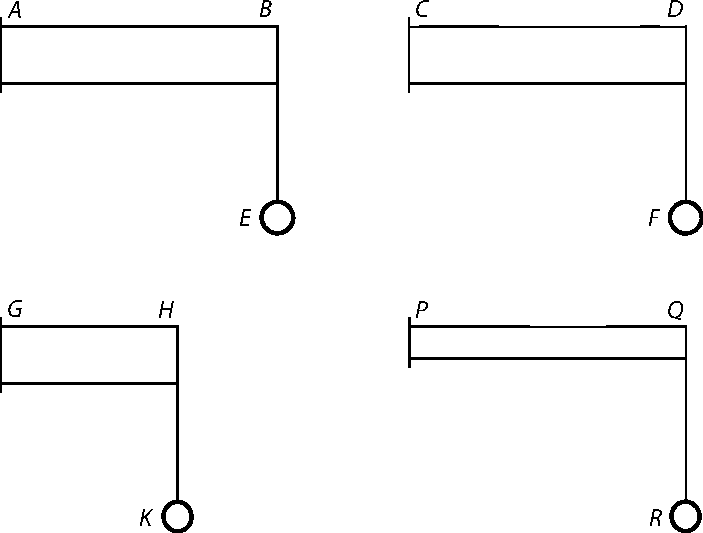
\includegraphics[width=0.68\textwidth]{gesamttex/edit_VIII,3/images/LH_35_09_15_008-009_d1.pdf}}%
  \vspace{0.5em}
  \centerline{\lbrack\textit{Fig.~1}\rbrack}%
  \label{LH_35_09_15_008r_Fig.1}%
%
  \vspace{1.5em}%
%  \newpage%
%
%
%\pstart
%\hspace{-8mm}dus $K$ est ad
%\edtext{pondus $F,$\protect\index{Sachverzeichnis}{pondus tendens} in ratione composita ex}{%
%\lemma{pondus}\Bfootnote{%
%\hspace{-0,5mm}$F,$
%\textit{(1)}~ut
%\textit{(2)}~in ratione composita ex%
%~\textit{L}}}
%$GH$ ad $CD$ et tensione ipsius $GH$ ad tensionem ispius $CD.$\protect\index{Sachverzeichnis}{tensio chordae}
%\pend
\pstart%
Ergo%
% !!!!! ACHTUNG GETRIXT !!!!! Nachfolgende C-footnote sollte eigentlich an Fig.~1 hängen!
\edtext{}{\lemma{\hspace*{1,6mm}\lbrack\textit{Fig.~1}\rbrack}\killnumber%
\Cfootnote{Zum Diagramm gehört auch die gestr. Zeichnung einer ähnlichen fünften Saite $LM,$
an der ein Gewicht $N$ hängt.}}%
\textso{ duae chordae similes diversarum}%
\protect\index{Sachverzeichnis}{chorda tensa}%
\protect\index{Sachverzeichnis}{tensio chordae}%
\protect\index{Sachverzeichnis}{pondus sustentans}%
\edtext{\textso{ tensionum ponderibus sustentantur,
quae sunt}}{%
\lemma{\textso{tensionum}}\Bfootnote{%
\textit{(1)}~sunt % \textso{}
\textit{(2)}~\textso{ponderibus sustentantur, quae sunt}%
~\textit{L}}}%
\textso{ in composita ratione longitudinum et}%
\edtext{\textso{ tensionum.}%
\protect\index{Sachverzeichnis}{longitudo chordae}\protect\index{Sachverzeichnis}{tensio chordae}
\newline%
%
\indent%
Sit alia chorda\protect\index{Sachverzeichnis}{chorda tensa}}{%
\lemma{\textso{tensionum.}}\Bfootnote{% \hspace*{-0,5mm} \textso{}
\textit{(1)}~Et duae chordae similes et aequales ponderibus sustentantur qu\protect\index{Sachverzeichnis}{pondus sustentans}
\textit{(2)}~Sit alia chorda%
~\textit{L}}}
tenuior \textit{PQ}
tensa pondere \textit{R}\protect\index{Sachverzeichnis}{pondus tendens}
aequalis longitudine\protect\index{Sachverzeichnis}{longitudo chordae} ipsis \textit{CD}
\edtext{et \textit{AB}
et aequalis}{%
\lemma{et}\Bfootnote{%
\hspace{-0,5mm}$AB$
\textit{(1)}~cum sint
\textit{(2)}~et aequalis%
~\textit{L}}}
tensione\protect\index{Sachverzeichnis}{tensio chordae} ipsi \textit{AB},
erit \textit{R} ad \textit{E} ut quadratum crassitiei ipsius \textit{PQ}\protect\index{Sachverzeichnis}{crassities chordae}
ad quadratum crassitiei ipsius \textit{AB},\protect\index{Sachverzeichnis}{crassities chordae}
est autem \textit{E} ad \textit{F} ut tensio ipius \textit{AB} seu ipsius \textit{PQ} ad tensionem ipsius \textit{CD}.%
\protect\index{Sachverzeichnis}{tensio chordae}
Ergo \textit{R} est ad \textit{F} in ratione composita
\edtext{ex ratione quadrati}{%
\lemma{ex}\Bfootnote{%
\textit{(1)}~rationibus quadratorum
\textit{(2)}~ratione quadrati%
~\textit{L}}}
a \edtext{crassitie\protect\index{Sachverzeichnis}{crassities chordae}
\textit{PQ} ad quadratum}{%
\lemma{crassitie}\Bfootnote{%
\hspace{-0,5mm}$PQ$ ad
\textit{(1)}~rati
\textit{(2)}~quadratum%
~\textit{L}}}
a crassitie\protect\index{Sachverzeichnis}{crassities chordae}
\edtext{\textit{CD} et tensionis}{%
\lemma{$CD$}\Bfootnote{%
\hspace{-0,5mm}et
\textit{(1)}~longit
\textit{(2)}~tensionis%
~\textit{L}}}
ipsius \textit{PQ} ad tensionem\protect\index{Sachverzeichnis}{tensio chordae}
\edtext{ipsius \textit{CD}.
Seu\textso{ chordarum ejusdem longitudinis}\protect\index{Sachverzeichnis}{longitudo chordae}%
\textso{ pondera sustentantia}\protect\index{Sachverzeichnis}{pondus sustentans}%
\textso{ }sunt%
\textso{ in duplicata ratione crassitierum}\protect\index{Sachverzeichnis}{crassities chordae}%
\textso{ et simplici tensionum.}\protect\index{Sachverzeichnis}{tensio chordae}}{%
\lemma{ipsius}\Bfootnote{% \hspace*{-0,5mm}
$CD$.
\textit{(1)}~Seu si chordae aequales sint diversarum crassitierum et tensionum
\textit{(2)}~Seu \textso{chordarum} \lbrack...\rbrack\ \textso{simplici tensionum.}%
~\textit{L}}}
%
\lbrack8~v\textsuperscript{o}\rbrack % Blatt 8v
%
\pend%
\newpage
  \centerline{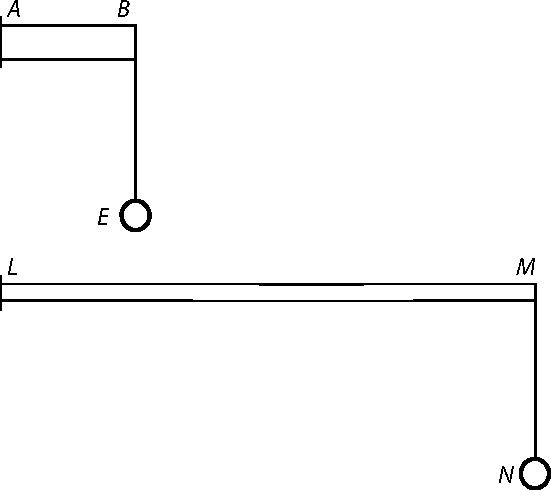
\includegraphics[width=0.52\textwidth]{gesamttex/edit_VIII,3/images/LH_35_09_15_008-009_d2.pdf}}%
  \vspace{0.3em}
  \centerline{\lbrack\textit{Fig.~2}\rbrack}%
  \label{LH_35_09_15_008r_Fig.2}%
  \vspace{1.5em}%%
  \count\Bfootins=1000
\count\Afootins=1000
\count\Cfootins=1000
\pstart%
Hinc%
\edlabel{LH_35_09_15_008v_vrws-1-1}
denique patet generalis regula ponderum,\protect\index{Sachverzeichnis}{regula ponderum}
nempe%
\textso{ Pondera chordas tendentia}\protect\index{Sachverzeichnis}{pondus tendens}%
\textso{ sunt in rationibus compositis ex simplici longitudinum,}\protect\index{Sachverzeichnis}{longitudo chordae}%
\textso{ simplici tensionum,}\protect\index{Sachverzeichnis}{tensio chordae}%
\textso{ et duplicata }%
\edtext{\textso{crassitierum.}\protect\index{Sachverzeichnis}{crassities chordae}%
\edlabel{LH_35_09_15_008v_vrws-1-2}
Si materia\protect\index{Sachverzeichnis}{materia chordae} una alia solidior sit%
\lbrack,\rbrack\
perinde est ac si una alia crassior esset.
Hinc%
\edlabel{LH_35_09_15_008r_reggenpond-1}
generaliter colligi potest:%
\textso{ Vires}\protect\index{Sachverzeichnis}{vis tendens}%
\textso{ esse in ratione corporum et tensionum.}%
\edlabel{LH_35_09_15_008r_reggenpond-2}\protect\index{Sachverzeichnis}{tensio chordae}
\newline%
%
\indent%
Si%
\edlabel{LH_35_09_15_008v_kndsz-1}%
\edtext{}{{\xxref{LH_35_09_15_008v_kndsz-1}{LH_35_09_15_008v_kndsz-2}}{%
\lemma{Si \lbrack...\rbrack\ dimidia}%
\Cfootnote{Die Textänderungen führen zu einem Konditionalgefüge,
dem der Haupt\-satz fehlt.}}}
\edtext{chorda $AB$\protect\index{Sachverzeichnis}{chorda tensa}}{%
\lemma{Si chorda $AB$}\Cfootnote{%
Siehe \lbrack\textit{Fig.~2}\rbrack.}}
magis}{%
\lemma{\textso{crassitierum.}}\Bfootnote{%
\hspace{-0,5mm}\textbar~Si materia \lbrack...\rbrack\ \textso{et tensionum.} \textit{erg.}~\textbar\
\textit{(1)}~Hinc ut
\textit{(2)}~Si chorda
\textit{(a)}~ad dupl
\textit{(b)}~$AB$ magis
\textit{L}}}
tendatur\lbrack,\rbrack\
\edtext{nempe ex longitudine $AB$ in longitudinem\protect\index{Sachverzeichnis}{longitudo chordae}}{%
\lemma{nempe}\Bfootnote{%
\textit{(1)}~in longitudinem
\textit{(2)}~ex longitudine $AB$ in longitudinem%
~\textit{L}}}
\edtext{majorem $LM$
quae sit ad $AB$ in ratione duplicata crassitierum,\protect\index{Sachverzeichnis}{crassities chordae}
seu exempli gratia quadrupla ipsius $AB,$
si crassities\protect\index{Sachverzeichnis}{crassities chordae}
tensione\protect\index{Sachverzeichnis}{tensio cordae} facta sit dimidia.%
\edlabel{LH_35_09_15_008v_kndsz-2}%
}{%
\lemma{majorem}\Bfootnote{%
\textit{(1)}~$CD$
\textit{(2)}~$LM$
\textit{(a)}~quae sit quadrupla ipsius $AB,$ erit crassities subdupla.
\textit{(b)}~quae sit ad $AB$ in \lbrack...\rbrack\ sit dimidia.%
~\textit{L}}}
Ergo cum ratio longitudinis\protect\index{Sachverzeichnis}{longitudo chordae}
sit ita semper reciproca
% ******
\edtext{rationis duplicatae crassitierum,\protect\index{Sachverzeichnis}{crassities chordae}
et generaliter
% \edtext{}{\lemma{generaliter}\Bfootnote{\textit{erg.~L}}}
ratio ponderum\protect\index{Sachverzeichnis}{pondus tendens}
\lbrack sit\rbrack\
in rationibus compositis ex simplici longitudinum,\protect\index{Sachverzeichnis}{longitudo chordae}
simplici tensionum\protect\index{Sachverzeichnis}{tensio chordae} et duplicata
% \edtext{}{\lemma{tensionum et}\Bfootnote{%
% \textit{(1)}~duplici
% \textit{(2)}~duplicata~\textit{L}}}
crassitierum,\protect\index{Sachverzeichnis}{crassities chordae}%
\textso{ }%
\edtext{\textso{per praecedentem\lbrack,\rbrack\ }%
}{\lemma{\textso{per praecedentem}\,}\Cfootnote{%
Siehe S.~\refpassage{LH_35_09_15_008v_vrws-1-1}{LH_35_09_15_008v_vrws-1-2}.}}%
% \textso{ }%
manifestum est hoc loco rationes duas\lbrack,\rbrack\
simplicem longitudinum\protect\index{Sachverzeichnis}{longitudo chordae}
(\phantom)\hspace*{-1.2mm}%
quae est reciproca duplicatae crassitierum hoc loco%
\phantom(\hspace*{-1.2mm})
et ipsam duplicatarum
% \edtext{}{\lemma{ipsam}\Bfootnote{%
% \textit{(1)}~duplicatam
% \textit{(2)}~duplicatarum~\textit{L}}}
crassitierum\protect\index{Sachverzeichnis}{crassities chordae}%
\lbrack,\rbrack\
sese invicem destruere,
nam rationes directae et reciprocae invicem compositae se destruunt,
faciuntque rationes aequalitatis.
Ergo restat sola ratio tensionum\protect\index{Sachverzeichnis}{tensio chordae}
destructis longitudinibus\protect\index{Sachverzeichnis}{longitudo chordae}
et crassitiebus\protect\index{Sachverzeichnis}{crassities chordae}%
\lbrack,\rbrack\
% ******
adeoque erunt pondera\protect\index{Sachverzeichnis}{pondus tendens}
ut tensiones.\protect\index{Sachverzeichnis}{tensio chordae}}{%
\lemma{rationis}\Bfootnote{% \hspace*{-0,5mm}
\textbar~duplicatae \textit{erg.}~%
\textbar\ crassitierum,
\textit{(1)}~sese
\textit{(a)}~restituent
\textit{(b)}~destruent
\textit{(2)}~et
\textbar~generaliter \textit{erg.}~%
\textbar\ ratio ponderum
\textbar~sint \textit{ändert Hrsg.}~%
\textbar\ in rationibus \lbrack...\rbrack\ tensionum et
\textit{(a)}~duplici
\textit{(b)}~duplicata
crassitierum, \textso{per} \lbrack...\rbrack\ loco\phantom(\hspace*{-1.2mm}) et ipsam
\textit{(aa)}~duplicatam
\textit{(bb)}~duplicatarum crassitierum sese \lbrack...\rbrack\
pondera ut tensiones.%
~\textit{L}}}
Cumque semper in ejusdem chordae\protect\index{Sachverzeichnis}{tensio chordae}
\edtext{tensione diversos ejus status\protect\index{Sachverzeichnis}{status tensionis} comparando sint}{%
\lemma{tensione}\Bfootnote{%
\textit{(1)}~sint
\textit{(2)}~diversos ejus status comparando sint%
~\textit{L}}}
longitudines\protect\index{Sachverzeichnis}{longitudo chordae}
in reciproca crassitierum\protect\index{Sachverzeichnis}{crassities chordae}
% \edtext{\lbrack ratione\rbrack}{%
% \lemma{ratione}\Bfootnote{\textit{erg. Hrsg.}}}
duplicata\lbrack,\rbrack\ semper
\edtext{se destruent}{%
\lemma{se}\Bfootnote{%
\textit{(1)}~restituent
\textit{(2)}~destruent%
~\textit{L}}}
hae duae rationes,
\edtext{adeoque:}{%
\lemma{adeoque:}\Bfootnote{%
\textit{(1)}~In
\textit{(2)}~\textso{Pondera}%
~\textit{L}}}%
\textso{ Pondera }\edtext{\textso{chordam tendentia}\protect\index{Sachverzeichnis}{pondus tendens}%
\textso{ sunt ut tensiones.}\protect\index{Sachverzeichnis}{tensio chordae}}{%
\lemma{\textso{chordam}}\Bfootnote{%
\textit{(1)}~\textso{tensio}
\textit{(2)}~\textso{tendentia sunt ut tensiones.}%
~\textit{L}}}
% > > > >
% ? ? ? ?
\pend%
%  \newpage%
%%
%%
%  %\vspace*{0.0em}%
%  \centerline{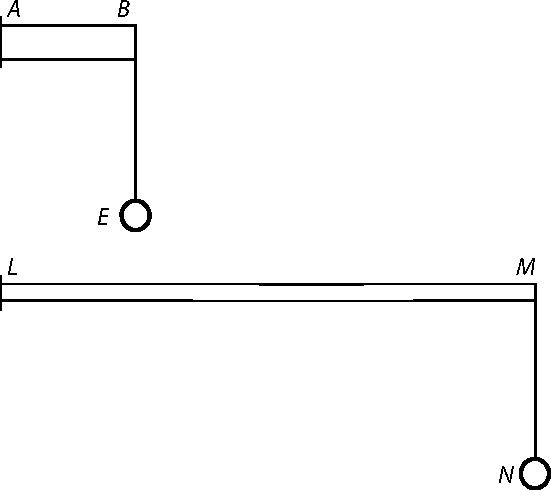
\includegraphics[width=0.52\textwidth]{gesamttex/edit_VIII,3/images/LH_35_09_15_008-009_d2.pdf}}%
%  \vspace{0.3em}
%  \centerline{\lbrack\textit{Fig.~2}\rbrack}%
%  \label{LH_35_09_15_008r_Fig.2}%
%  \vspace{1.0em}%%
%%  \newpage
%%
%
\pstart%
Porro\edlabel{LH_35_09_15_008v_siluaekg-1}
Tensiones ejusdem chordae\protect\index{Sachverzeichnis}{tensio chordae} sunt inter se
\edtext{ut mutationes,\protect\index{Sachverzeichnis}{mutatio chordae}
mutationes autem vel secundum crassities,\protect\index{Sachverzeichnis}{crassities chordae}
vel secundum longitudines\protect\index{Sachverzeichnis}{longitudo chordae} sumi possunt,}{%
\lemma{ut}\Bfootnote{%
\hspace{-0,5mm}mutationes,
\textit{(1)}~sunt autem
\textit{(2)}~mutationes autem \lbrack...\rbrack\ sumi possunt,%
~\textit{L}}}
sed utroque modo res
\edtext{eadem redit,}{%
\lemma{eadem}\Bfootnote{%
\hspace{-0,5mm}\textbar~enim \textit{streicht Hrsg.}~\textbar\ redit,
\textit{L}}}
%
altera enim alteram continet.
Si secundum crassities\protect\index{Sachverzeichnis}{crassities chordae} sumantur,
sumendae erunt bases\protect\index{Sachverzeichnis}{basis chordae}
crassitierum, non diametri,\protect\index{Sachverzeichnis}{diameter chordae}
\edtext{itaque mutationes\protect\index{Sachverzeichnis}{mutatio chordae} sunt}{%
\lemma{itaque}\Bfootnote{%
\textit{(1)}~mutationes sunt
\textit{(2)}~mutationes sunt%
~\textit{L}}}
ut longitudines,\protect\index{Sachverzeichnis}{longitudo chordae}
vel \edtext{etiam ut tenuitatum\protect\index{Sachverzeichnis}{tenuitas chordae}
(\phantom)\hspace*{-1.2mm}%
seu reciprocarum crassitierum\protect\index{Sachverzeichnis}{crassities chordae}%
\phantom(\hspace*{-1.2mm})}{%
\lemma{etiam}\Bfootnote{% \hspace*{-0,5mm}
ut
\textit{(1)}~crassiti
\textit{(2)}~tenuitatum (\phantom)\hspace*{-1.2mm}seu reciprocarum crassitierum\phantom(\hspace*{-1.2mm})%
~\textit{L}}}
bases.\protect\index{Sachverzeichnis}{basis chordae}%
\textso{ Si jam ponatur chordam semel tensam}\protect\index{Sachverzeichnis}{chorda tensa}%
\textso{ non ideo reddi tensu difficiliorem, neque }%
\edtext{\textso{faciliorem }%
%
\lbrack9~r\textsuperscript{o}\rbrack\ % Blatt 9r
%
seu ejusdem chordae tensae\protect\index{Sachverzeichnis}{chorda tensa}
diversos status\protect\index{Sachverzeichnis}{status tensionis}
inter se invicem differre
solis tenuitatum\protect\index{Sachverzeichnis}{tenuitas chordae}
basibus\protect\index{Sachverzeichnis}{basis chordae}
ac longitudinibus,\protect\index{Sachverzeichnis}{longitudo chordae}}{%
\lemma{\textso{faciliorem}}\Bfootnote{%
\textit{(1)}~seu
\textit{(a)}~chordas tensas
\textit{(b)}~chordam tensam
\textit{(c)}~solummo
\textit{(d)}~\textbar~eandem \textit{streicht Hrsg.}~\textbar\
\lbrack9~r\textsuperscript{o}\rbrack\
\textit{(2)}~seu ejusdem \lbrack...\rbrack\ differre solis
\textit{(a)}~basium
\textit{(b)}~tenuitatum basibus ac longitudinibus,%
~\textit{L}}}
\edtext{quae duae res
(\phantom)\hspace*{-1.2mm}%
tenuitates\protect\index{Sachverzeichnis}{tenuitas chordae}
secundum bases\protect\index{Sachverzeichnis}{basis chordae}
sumptae et longitudines\protect\index{Sachverzeichnis}{longitudo chordae}%
\phantom(\hspace*{-1.2mm})
se}{%
\lemma{quae}\Bfootnote{%
\textit{(1)}~se
\textit{(2)}~res
\textit{(3)}~duae res \lbrack...\rbrack\ longitudines\phantom(\hspace*{-1.2mm}) se%
~\textit{L}}}
invicem compensant;
sequitur Tensiones\protect\index{Sachverzeichnis}{tensio chordae} seu
\edtext{impetus restituentes\protect\index{Sachverzeichnis}{impetus restituens}
qui chordae incumbunt,}{%
\lemma{impetus}\Bfootnote{%
\textit{(1)}~qui chordae incumbunt
\textit{(2)}~restituentes qui chordae incumbunt,%
~\textit{L}}}
fore ut longitudines,\protect\index{Sachverzeichnis}{longitudo chordae}
seu fore ut tenuitatum\protect\index{Sachverzeichnis}{tenuitas chordae}
bases,\protect\index{Sachverzeichnis}{basis chordae}
et necesse est causam restituentem\protect\index{Sachverzeichnis}{causa restituens}\lbrack,\rbrack\
quaecumque ea
\edtext{sit\lbrack,\rbrack\
proportione}{%
\lemma{sit}\Bfootnote{%
\textit{(1)}~secundum
\textit{(2)}~proportione%
~\textit{L}}}
longitudinum\protect\index{Sachverzeichnis}{longitudo chordae} agere.%
\edlabel{LH_35_09_15_009r_siluaekg-2}
An autem \protect\index{Sachverzeichnis}{hypothesis}haec%
\textso{ Hypothesis }%
consentiat phaenomenis,\protect\index{Sachverzeichnis}{phaenomenon}
\edtext{ex consequentiis\protect\index{Sachverzeichnis}{consequens} videbimus.}{%
\lemma{ex consequentiis videbimus}\Cfootnote{%
Siehe N.~8\textsubscript{3}.}}
\pend%
%\newpage%
%
\pstart%
Hinc%
\edlabel{LH_35_09_15_009r_tensutlong-1}
manifestum etiam est:%
\textso{ Pondera eandem chordam tendentia}\protect\index{Sachverzeichnis}{pondus tendens}%
\textso{ esse ut longitidines,}\protect\index{Sachverzeichnis}{longitudo chordae}%
\edlabel{LH_35_09_15_009r_tensutlong-2}
seu%
\textso{ ut tenuitatum}\protect\index{Sachverzeichnis}{tenuitas chordae}%
\textso{ bases }%
seu reciproce ut bases\protect\index{Sachverzeichnis}{basis chordae}
crassitierum.\protect\index{Sachverzeichnis}{crassities chordae}%
\edlabel{LH_37_09_15_012v_udzfgouzdfg-2}
\pend%
%
\pstart%
Nunc%
\edlabel{LH_35_09_15_009r_vrwsltzt-1}
etiam\textso{ Tempora restitutionum}\protect\index{Sachverzeichnis}{tempus restitutionis}%
\textso{ consideremus.}
Assumsimus
\edtext{autem velut primum principium}{%
\lemma{autem}\Bfootnote{%
\textit{(1)}~jam
\textit{(2)}~velut primum principium%
~\textit{L}}}
\edtext{supra}{%
\lemma{supra}\Cfootnote{N.~8\textsubscript{1}, S.~\refpassage{LH_35_09_15_007v_vrws2-1}{LH_35_09_15_007v_vrws2-2}.}}%
\textso{ duas chordas similes aequales et }%
\edtext{\textso{aeque tensas,}\protect\index{Sachverzeichnis}{chorda tensa}%
\textso{ vel}}{%
\lemma{\textso{aeque}}\Bfootnote{%
\hspace*{-1,1mm}\textso{ tensas,}
\textit{(1)}~seu
\textit{(2)}~vel%
~\textit{L}}}%
\textso{ iisdem positis eodem pondere tensas,}\protect\index{Sachverzeichnis}{pondus tendens}%
\textso{ restitui eodem tempore.}\protect\index{Sachverzeichnis}{tempus restitutionis}
Nihil enim
\edtext{aliud hoc est quam}{%
\lemma{aliud}\Bfootnote{%
\textit{(1)}~es
\textit{(2)}~quam
\textit{(3)}~hoc est quam%
~\textit{L}}}
exemplum axiomatis\protect\index{Sachverzeichnis}{axioma} generalis,
quod si nullum sit discrimen in antecedentibus,\protect\index{Sachverzeichnis}{discrimen in antecedentibus}
nullum etiam futurum sit discrimen in
\edtext{consequentibus.\protect\index{Sachverzeichnis}{discrimen in consequentibus}%
\edlabel{LH_35_09_15_009r_vrwsltzt-2}%
\newline%
\indent%
\textso{Ejusdem chordae}\protect\index{Sachverzeichnis}{chorda tensa}}{%
\lemma{consequentibus.}\Bfootnote{%
\textit{(1)}~Si duae sint chordae
\textit{(2)}~\textso{Ejusdem chordae}%
~\textit{L}}}%
\textso{ partes simul }%
\edtext{\textso{restituuntur }\protect\index{Sachverzeichnis}{restitutio chordae}cum tota,
quamdiu ei cohaerent,}{%
\lemma{\textso{restituuntur}}\Bfootnote{%
\textit{(1)}~cum tota,
\textit{(2)}~cum tota, quamdiu ei cohaerent,%
~\textit{L}}}
quia chordae quaelibet pars semper aeque tensa est.\protect\index{Sachverzeichnis}{chorda tensa}
\pend%
%
%
%  \newpage%  !!!!! Rein vorläufig !!!!!
  \vspace{2.0em}%
  \centerline{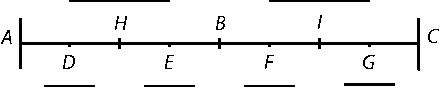
\includegraphics[width=0.42\textwidth]{gesamttex/edit_VIII,3/images/LH_35_09_15_008-009_d3.pdf}}%\\
  \vspace{0.5em}
  \centerline{\lbrack\textit{Fig.~3, gestr.}\rbrack}%
%  \newpage
  \vspace{1.5em}%
%
%
\pstart%
\noindent%
\lbrack\textit{Nachfolgend kleingedruckter Text in L gestrichen:}\rbrack\
\pend%
\vspace{0.5em}%
%
\footnotesize%
\pstart%
Si chorda tensa $ABC$\protect\index{Sachverzeichnis}{chorda tensa}
et utrinque in $A$ et $B$ firmiter annexa
eodem momento\protect\index{Sachverzeichnis}{momentum temporis}
secetur in tribus punctis $A.$ $B.$ $C$
manifestum est eodem tempore chordam $AB$ reductum iri\protect\index{Sachverzeichnis}{reductio chordae} in
\edtext{$DE,$ et $BC$ in $FG,$}{%
\lemma{$DE,$}\Bfootnote{%
\hspace{-0,5mm}et
\textit{(1)}~$FG$
\textit{(2)}~$BC$ in $FG,$%
~\textit{L}}}
et fore $AD$ aequ. $BE$ aequ. $BF$ aequ. $GC,$
et fore $DE$ ad $AB,$ ut $FG$ ad $BC.$
Si vero chorda tota in extremitatum secetur vel dimittatur
reducetur\protect\index{Sachverzeichnis}{reductio chordae} in $HI,$ eruntque,
\edtext{$AH$ aequ. $CI.$}{%
\lemma{$AH$}\Bfootnote{%
\hspace{-0,5mm}aequ. $CI.$
\textit{erg.~L}}}
$AC : HI \squaredots AB : DE \squaredots BC : FG.$
Hinc apparet \normalsize{\lbrack\textit{Text bricht ab.}\rbrack\ }
%
\lbrack9~v\textsuperscript{o}\rbrack\ % Blatt 9v
%
%
\pend%
\vspace{0.5em}
%
\normalsize%
\pstart%
\textso{Duarum}\edlabel{LH_35_09_15_009v_utlong-1}\edlabel{LH35_09_15_009v_quominoreocitius-1}\edlabel{LH35_09_15_009v_freqzulaeng-1}%
\textso{ chordarum similium et aeque tensarum,}\protect\index{Sachverzeichnis}{chorda tensa}%
\textso{ sed inaequalium minor celerius restituitur.}\protect\index{Sachverzeichnis}{restitutio chordae}\edlabel{LH35_09_15_009v_freqzulaeng-2}
\edtext{Nam omnium minima\protect\index{Sachverzeichnis}{portio chordae omnium minima}
seu infinite parva chordae tensae portio\protect\index{Sachverzeichnis}{portio chordae infinite parva}
restitueretur momento.%
\protect\index{Sachverzeichnis}{restitutio chordae}\protect\index{Sachverzeichnis}{momentum temporis}
Causa est,\protect\index{Sachverzeichnis}{causa}
quia et per spatium\protect\index{Sachverzeichnis}{spatium restitutionis} infinite parvum decurrit.\edlabel{LH35_09_15_009v_quominoreocitius-2}}{%
\lemma{Nam \lbrack...\rbrack\ decurrit}\Cfootnote{%
Gleiche Beweisführung in N.~9, S.~\refpassage{LH_35_09_15_005r_quominoreocitius-1}{LH_35_09_15_005r_quominoreocitius-2}.}}
\pend%
  \vspace{3.0em}%
  \centerline{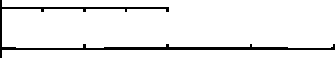
\includegraphics[width=0.48\textwidth]{gesamttex/edit_VIII,3/images/LH_35_09_15_008-009_d4.pdf}}%
  \vspace{0.5em}%
  \centerline{\lbrack\textit{Fig.~4}\rbrack}%
%\newpage%
%
\count\Bfootins=1000
\count\Afootins=1000
\count\Cfootins=1000
\pstart%
\textso{Chordarum}%
\textso{ similium aeque tensarum}\protect\index{Sachverzeichnis}{chorda tensa}%
\textso{ restitutiones}\protect\index{Sachverzeichnis}{restitutio chordae}%
\textso{ sunt ut }%
\edtext{\textso{longitudines.}\protect\index{Sachverzeichnis}{longitudo chordae}
Secetur utraque in partes infinite parvas\protect\index{Sachverzeichnis}{pars chordae infinite parva}
numero infinitas, aequales,
ipsae hae particulae ponantur rigidae.\protect\index{Sachverzeichnis}{particula chordae rigida}
Erunt impetus tendentes\protect\index{Sachverzeichnis}{impetus tendens}
tot quot particulae.\protect\index{Sachverzeichnis}{particula chordae}
Erunt et impetus\protect\index{Sachverzeichnis}{impetus tendens}
aequales, et omnia alia eadem,
\lbrack sed\rbrack\
tantum percurrendum majus spatium\protect\index{Sachverzeichnis}{spatium restitutionis}
cuilibet puncto, nempe in ratione chordarum.
Ergo tempora\protect\index{Sachverzeichnis}{tempus restitutionis} ut chordae.
Clarior res erit,
si pro una longiore sumas unum minutum secundum temporis,
pro altera breviore dimidium.
Sed haec
\edtext{alias}{\lemma{alias}\Cfootnote{%
Es ist nicht ersichtlich, worauf Leibniz anspielt.
%% Möglicherweise in N.~??A10\textsubscript{5}, S.~\refpassage{LH_35_09_15_015v_recprtens-1}{LH_35_09_15_015v_recprtens-2}.???
%% Siehe FN auf S. 39: Die dortigen Hinweise könnten auch hier gelten.
}}
exactius demonstranda.
Interim assumamus saltem hanc propositionem\protect\index{Sachverzeichnis}{propositio}
ut circiter veram.
Nam et
\edtext{supra}{\lemma{supra}\Cfootnote{%
N.~8\textsubscript{1}, S.~\refpassage{LH_35_09_15_007v_vrws2-1}{LH_35_09_15_007v_vrws2-2}.}}
eam partialiter\lbrack,\rbrack\
argumento\protect\index{Sachverzeichnis}{argumentum} tamen eodem redeunte\lbrack,\rbrack\
confirmavimus,
et assumturos nos diximus.%
\edlabel{LH_35_09_15_009v_utlong-2}%
}{%
\lemma{\textso{longitudines.}}\Bfootnote{%
\textit{(1)}~Quid si
\textit{(2)}~Dividatur utraque
\textit{(3)}~Dividantur
\textit{(a)}~singul 
\textit{(b)}~in partes
\textit{(aa)}~par
\textit{(bb)}~infinite parvas aequales
\textit{(4)}~Aequisecentur singulae in numerum
\textit{(5)}~Secetur et hae et illae in
\textit{(a)}~partes infinite parvas
\textit{(b)}~infinitibus
\textit{(c)}~infinitas numero aequales,
sitque pars una unius ad unam alterius ut tota ad totam,
patet partes majoris et minoris eodem impetu percuti,
intelliguntur enim singulae hae partes rigidae nec tendibiles,
ideoque tot erunt impetus tendentes, quot particulae tales. Et
\textit{(aa)}~impetuum numerus erit
\textit{(bb)}~impetus numeri erunt ut magnitu
% Stufe 6 = gültiger Text
\textit{(6)}~Secetur utraque \lbrack...\rbrack\ infinitas, aequales,
\textit{(a)}~erunt
\textit{(b)}~ipsae hae particulae \lbrack...\rbrack\ tot quot particulae.
\textit{(aa)}~Ergo impetus
\textit{(bb)}~Erunt et impetus aequales,
\textit{(aaa)}~ergo
\textit{(bbb)}~sed tantum percurrend
\textit{(ccc)}~et
\textit{(ddd)}~et omnia alia eadem,
\textbar~sed \textit{erg. Hrsg.}~%
\textbar\ tantum percurrendum
\lbrack...\rbrack\ tempora ut chordae.
\textit{(aaaa)}~Clarjus
\textit{(bbbb)}~Clarior res erit, si pro una
\textbar~longiore \textit{erg.}~%
\textbar\ sumas
\textit{(aaaaa)}~unam horam, pro
\textit{(bbbbb)}~unum
\textbar~minutum \textit{erg.}~%
\textbar\ secundum
\textbar~temporis \textit{erg.}~%
\textbar~, pro altera
\textit{(aaaaa-a)}~alterum
\textit{(bbbbb-b)}~breviore dimidium
\textit{(aaaaa-aa)}~, ejus
\textit{(bbbbb-bb)}~. Sed haec
\textit{(aaaaa-aaa)}~omnia non sunt satis exacte demonstrata.
Assumamus saltem hanc propositionem
\textbar~interim \textit{erg.}~%
\textbar\ ut circiter veram.
\textit{(bbbbb-bbb)}~alias exactius demonstranda.
\lbrack...\rbrack\
ut circiter veram.
\textit{(aaaaa-aaaa)}~Quemadmodum
\textit{(bbbbb-bbbb)}~Nam et supra \lbrack...\rbrack\ nos diximus.%
~\textit{L}}}
\pend%
%
\pstart%
\edtext{\textso{Chordarum}\edlabel{LH_35_09_15_009v_crassitiessuperflua-1}%
\textso{ aeque longarum et aeque tensarum,}\protect\index{Sachverzeichnis}{chorda tensa}%
\textso{ sed diversae }%
\edtext{\textso{crassitiei}\protect\index{Sachverzeichnis}{crassities chordae}%
\textso{ isochronae sunt}}{%
\lemma{\textso{crassitiei\,}}\Bfootnote{%
\textit{(1)}~\textso{chordae sunt\,}
\textit{(2)}~\textso{isochronae sunt\,}%
~\textit{L}}}%
\textso{ restitutiones,}\protect\index{Sachverzeichnis}{restitutio isochrona}
perinde est enim ac si plures chordae colligatae
\edlabel{LH_35_09_15_009v-gstr-1}essent.\edlabel{LH_35_09_15_009v_crassitiessuperflua-2}%
}{\lemma{\textso{Chordarum} \lbrack...\rbrack\ essent}\Cfootnote{%
Siehe \cite{00044}H.~\textsc{Fabri}, \textit{Physica}, tract.~III, lib.~II, prop.~223; 224 (Bd.~II, Lyon 1670, S.~215b; 216a; 216b).}}%
%
\edtext{}{{\xxref{LH_35_09_15_009v-gstr-1}{LH_35_09_15_009v-gstr-2}}{%
\lemma{essent}\Bfootnote{%
\textit{(1)}~velut
\textit{(2)}~. Idque est%
~\textit{L}}}}
%
\pend%
\count\Bfootins=1200
\count\Afootins=1000
\count\Cfootins=1200
\vspace{0.5em}
\pstart%
\noindent%
\lbrack\textit{Nachfolgend kleingedruckter Text in L gestrichen:}\rbrack\
\pend%
\vspace*{0.5em}%
\footnotesize%
\pstart
Idque
\edlabel{LH_35_09_15_009v_schd3.2-1}%
est%
\edlabel{LH_35_09_15_009v-gstr-2}
sive duae chordae aeque tensae
\edtext{similes}{%
\lemma{similes}\Bfootnote{\textit{erg.~L}}}
inaequales omnino dimittantur
\edtext{ad statum naturalem,\protect\index{Sachverzeichnis}{status naturalis}}{%
\lemma{ad}\Bfootnote{%
\hspace{-0,5mm}statum naturalem \textit{erg.~L}}}
sive ad eandem tensionem novam
\edtext{pulsentur
atque inde dimissae redeant ad tensionem\protect\index{Sachverzeichnis}{tensio chordae} priorem,
restitutiones erunt ut}{%
\lemma{pulsentur}\Bfootnote{%
\hspace{-0,5mm}\textbar~atque inde \lbrack...\rbrack\ tensionem priorem, \textit{erg.}~\textbar\
\textit{(1)}~isochronae
\textit{(2)}~restitutiones
\textit{(a)}~ut
\textit{(b)}~erunt ut%
~\textit{L}}}
longitudines reciprocae.
%
Revera enim semper a tensione\protect\index{Sachverzeichnis}{tensio chordae} nova restituuntur.
Et
\edtext{si}{%
\lemma{si}\Bfootnote{\textit{erg.~L}}}
restitutio\protect\index{Sachverzeichnis}{restitutio isochrona}
\edtext{ad totam}{%
\lemma{ad}\Bfootnote{%
\textit{(1)}~totum
\textit{(2)}~totam%
~\textit{L}}}
usque naturalem\protect\index{Sachverzeichnis}{tensio naturalis}
utrobique est isochrona\lbrack,\rbrack\
etiam restitutio a secunda tensione ad primam erit isochrona.%
\protect\index{Sachverzeichnis}{restitutio isochrona}
Item si haec est isochrona a
\edtext{tensione secunda}{%
\lemma{tensione}\Bfootnote{%
\textit{(1)}~pri
\textit{(2)}~secunda%
~\textit{L}}}
ad primam,
erit et a prima ad quandam minorem,
et ita semper usque minimam.
\newline%
\indent%
\edtext{Itaque generaliter:%
\textso{ restitutiones duarum chordarum similium inaequalium
aeque tensarum}\protect\index{Sachverzeichnis}{chorda tensa}%
\textso{ sunt isochronae.}\!\protect\index{Sachverzeichnis}{restitutio isochrona}%
\textso{ Ergo et ab eadem tensione}\protect\index{Sachverzeichnis}{tensio chordae}%
\textso{ ad nullam, seu ad statum }%
\edlabel{LH_35_09_15_009v_ende-1}%
\edtext{}{{\xxref{LH_35_09_15_009v_ende-1}{LH_35_09_15_009v_ende-2}}%
\lemma{\textso{naturalem.}}\Bfootnote{%
\hspace{-0,5mm}\textbar~Reductiones et \textit{gestr.}~%
\textbar\ \textso{Restitutiones}%
~\textit{L}}}%
\textso{naturalem.}\protect\index{Sachverzeichnis}{status naturalis}%
\edlabel{LH_35_09_15_009v_schd3.2-2}%
}{\lemma{\textit{Am Rand, ebenfalls gestrichen:}%
}\Afootnote{%
\footnotesize{%
Haec propositio\protect\index{Sachverzeichnis}{propositio} certa est ex praemissis.%
\protect\index{Sachverzeichnis}{praemissa}
Sed intelligitur duas illas chordas \normalsize{\lbrack\textit{Text bricht ab.}\rbrack}}}}%
\pend%
\vspace*{0.5em}%
%
\normalsize
\pstart%
\textso{Restitutiones}%
\edlabel{LH_35_09_15_009v_ende-2}\edlabel{LH_35_09_15_009v_restprsct-1}%
\textso{ ejusdem }%
\edtext{\textso{chordae tam omnimodae quam ad eandem usque tensionem,
si tensae}\protect\index{Sachverzeichnis}{chorda tensa}%
\textso{ fuerint praesectae}}{%
\lemma{\textso{chordae}}\Bfootnote{%
\textit{(1)}~\textso{ab eadem tensione ad eandem}
\textit{(2)}~\textso{tam omnimodae} \lbrack...\rbrack\ \textso{si tensae}
\textit{(a)}~\textso{porro}
\textit{(b)}~\textso{fuerint praesectae}%
~\textit{L}}}%
\textso{ sunt isochronae.}\edlabel{LH_35_09_15_009v_restprsct-2}\protect\index{Sachverzeichnis}{restitutio isochrona}
Cum enim spatium\protect\index{Sachverzeichnis}{spatium restitutionis}
tempore\protect\index{Sachverzeichnis}{tempus restitutionis} compensetur,
hanc
\edtext{assumsimus interim,}{%
\lemma{assumsimus interim}\Cfootnote{%
Siehe N.~8\textsubscript{1}, S.~\refpassage{LH_35_09_15_007v_vrws2-1}{LH_35_09_15_007v_vrws2-2}.}}
ut circiter veram.
Quia experimentis\protect\index{Sachverzeichnis}{experimentum} comprobatur.
%
\pend%
\count\Bfootins=1200
\count\Afootins=1200
\count\Cfootins=1200
%
\newpage% % % %    R e i n   v o r l ä u f i g    ! ! ! !
%
% ENDE DES STÜCKES auf Blatt 9v